\documentclass{template/openetcs_article}
%\documentclass{article}
%\usepackage[ascii]{inputenc}
%\usepackage[T1]{fontenc}
\usepackage[english]{babel}
\usepackage{amsmath}
\usepackage{amssymb,amsfonts,textcomp}
\usepackage{array}
\usepackage{supertabular}
\usepackage{hhline}
\usepackage{graphicx}
\makeatletter
\newcommand\arraybslash{\let\\\@arraycr}
\makeatother
\setlength\tabcolsep{1mm}
\renewcommand\arraystretch{1.3}
\newcounter{Ilustracin}
\renewcommand\theIlustracin{\arabic{Ilustracin}}
\title{openETCS}

%\setcounter{tocdepth}{3}
\usepackage{float}
\usepackage{hhline}
\usepackage{booktabs}
\usepackage{multirow}
\usepackage{color, colortbl}
\definecolor{myblue}{rgb}{0.6,.6,1}
\definecolor{mydarkblue}{rgb}{0,0,0.5}
\definecolor{mylightblue}{rgb}{0.8,0.8,1}
\usepackage{hyperref}
\hypersetup{colorlinks=true, linkcolor=mydarkblue, urlcolor=mydarkblue}

\usepackage[textwidth=2.7cm,textsize=scriptsize,linecolor=green!40,backgroundcolor=green!40]{todonotes}

\newcounter{mycommentcounter}
\newcommand{\mycomment}[2][]
{
\refstepcounter{mycommentcounter}%
\todo[color={red!100!green!33}]{
\textbf{[\uppercase{#1} \themycommentcounter]:} #2}
}


\usepackage{lipsum,url}
\graphicspath{{./template/}{.}{./images/}}
\begin{document}
\frontmatter
\project{openETCS}

%Please do not change anything above this line
%============================
% The document metadata is defined below

%assign a report number here
\reportnum{OETCS/WP1/D1.3.1}

%define your workpackage here
\wp{Work-Package 1: ``Management''}

%set a title here
\title{Project Quality Assurance Plan - Documentation control Process}

%set a subtitle here
%\subtitle{A template for short document. Adapted from report template.}

%set the date of the report here
\date{\today}

%define a list of authors and their affiliation here

\author{Ainhoa Gracia}

\affiliation{Avda. Zugazarte 8,6\\
  48930 Getxo \\
  Vizcaya, España}


% define the coverart
\coverart[width=350pt]{openETCS_EUPL}

%define the type of report
\reporttype{Description of work}




%=============================
%Do not change the next three lines
\maketitle
\tableofcontents
%\listoffiguresandtables
\newpage
%=============================

% The actual document starts below this line
%=============================


%Start here



%\begin{document}


\section*{Document History}

\begin{flushleft}
%\tablefirsthead{\hline Version & Date & Chapters modified & Reason & Name\\}

\tablehead{\hline \rowcolor{myblue} Version & Date & Chapters modified & Reason & Name\\}

\tabletail{}
\tablelasttail{}
\begin{supertabular}{m{1.1cm}m{1.8cm}m{2cm}m{7cm}m{2cm}lp{6cm}|}
\hline
0.1.0 &
22.08.2013 &
All &
First version &
Ainhoa Gracia (SQS)
\end{supertabular}
\end{flushleft}

\newpage

\section{Introduction}

\subsection[Introduction]{Purpose of the document}
The purpose of this procedure is to outline the process for openETCS Document Control in accordance with the Eclipse development process and CENELEC. 

This procedure describes:
\begin{itemize}
\item The methodology for ensuring that the documentation developed whiting the openETCS project is current and suitable for use by the Eclipse community, the project members and the key customers. This includes the process to be followed for:
\begin{itemize}
\item Document creation
\item Document review
\item Modification and update of documents (where necessary) that ensures the relevant experts or members of the community are consulted and given a genuine opportunity to provide input prior to approval
\item Identification of documents to ensure the most current versions are identifiable, legible and available at points of use
\item The prevention of unintended use of obsolete documents
\item Document approval prior to issue
\item Communication of approved new or modified documents to involved members of the community
\end{itemize}
\item The process for managing the openETCS documents shall be maintained in accordance with the project requirements, so it covers the needs identified in different phases of the project.
\end{itemize}

\subsection{Intended Audience}
This document applies to the whole development life-cycle of the project and it addresses all the author(s), product owners, commiters and users involved. This document should be available to all of them in read access mode and it provides guidance about the Documentation control process whenever it is needed. 

\subsection{Supporting documents}
\begin{center}
\begin{longtable}[H]{|m{2,5cm}m{2,5cm}m{9cm}|}
\caption{Supporting documents}\\

\hline \rowcolor{myblue} \multicolumn{1}{l}{Name} & \multicolumn{1}{l}{Path} & \multicolumn{1}{l}{Contents}\\ \hline 
\endfirsthead

\multicolumn{3}{c}%
{{\bfseries \tablename\ \thetable{} -- continued from previous page}} \\
\hline \rowcolor{myblue} \multicolumn{1}{l}{Name} & \multicolumn{1}{l}{Path} & \multicolumn{1}{l}{Contents}\\\hline
\endhead

\hline \hline
\endlastfoot

QA Plan & governance/ QA Plan & It defines the processes, methods and tools that will be used to develop the OpenETCS project
\\\hline
Revision Process & governance/ Review & This document presents the whole process to follow when documents need revision. It aims to provide a set of guidelines as technical instructions for each revision cycle launched that highlights the steps to take.
\\\hline
Review Process & governance/ Review & This document presents the whole process to follow when documents need review. It aims to provide a set of guidelines as technical instructions to be used whenever a review process is ongoing, or there are a set of issues reported that shall be considered. 
\\\hline
Change/Problem Management Process & governance/ Change-Problem Process & The main focus area of the document is the Change Request/Problem handling process which involves the detection and registration of Changes/Problems, followed by triage (classifying, prioritising and assigning incidents), change/problem resolution, closing and post-analysis.
\\\hline
SCMP & governance /SCMP & This document describes the applicable software configuration management directives which shall be applied by the software development team. Configuration Management (CM) is used to handle changes systematically so that a system 10 maintains its integrity over time. The Software Configuration Management Plan (SCMP) defines the procedures, techniques, and tools that are required to manage the software development, evaluate proposed changes, trace the status of changes, and to support an inventory of the system.
\\\hline
\end{longtable}
\end{center}

\subsection{Definitions and acronyms}
\begin{center}
\begin{longtable}{|m{3cm}m{11cm}|}
\caption{Definitions and acronyms}\\

\hline \rowcolor{myblue} \multicolumn{1}{|l}{\textbf{Abbreviation}} & \multicolumn{1}{l|}{\textbf{Meaning}} \\ \hline 
\endfirsthead

\multicolumn{2}{c}%
{{\bfseries \tablename\ \thetable{} -- continued from previous page}} \\
\rowcolor{myblue} \multicolumn{1}{|l}{\textbf{Abbreviation}} & \multicolumn{1}{l|}{\textbf{Meaning}} \\ \hline 
\endhead

\hline \hline
\endlastfoot

openETCS Documentation & It is important for the success of the openETCS project allowing for consistency and uniformity in applying the Eclipse Development process and follow the CENELEC standard. Typical documents of the project include plans, policies, procedures, guidelines and processes that define the objectives to approach and the way to do it.
\\\hline
Document control & The process established in this procedure to define controls needed for the management of openETCS documentation.
\\\hline
Document & Any document for which distribution and status are required to be kept current by the author(s) to ensure that authorised holders or key customers have the most up to date version available. It involves any Process, Instruction, Guidance and other supporting documents that are controlled / maintained under SCMP. Documents are maintained on gitHub and therefore, the documents are legible. Document numbers and revisions are assigned according to the Nomenclature guidance and they are assigned to ensure that documents are readily identifiable.
\\\hline
Active & A document that has been approved, controlled, and accessed and can be viewed on the gitHub.
\\\hline
Draft & An unapproved document that may be controlled and accessed by gitHub but that has been labelled as draft.
\\\hline
Obsolete & A document that has been superseded and will never be used again. Obsolete copies are safeguarded from inadvertent use in an “Obsolete” directory in the corresponding repository of gitHub.
\\\hline
Change &
the addition, modification, or removal of a configuration item (CI), product, or product component, and/or its associated elements
\\\hline
SCMP &
Software Configuration Management Plan. 
\\\hline
\end{longtable}
\end{center}

\section{Tools}
\begin{table}[H]
\begin{tabular}{|m{3cm}|m{11cm}|}
\hline
\rowcolor{myblue}
\multicolumn{2}{|c|}{Tools} \\\hline
GIT &
\begin{itemize}
\item \underline{GitHub}: A web-based hosting service for projects that use Git revision control system.
\item \underline{Issue Tracker (in GitHub)}: The issue tracker is integrated with the project's repository. Some of the features included are: the possibility of modifying tickets from within commit messages,
creating and applying labels to issues to assign to users or categorize, voting on issues that you want to see tackled, searching, sorting, and filtering, and keyboard shortcuts.
\end{itemize}
\\\hline
\end{tabular}
\caption{Tools}
\end{table}

\section{Documentation Control Process overview}

The Documentation control process describes how openETCS documents are controlled. Implementation of the corresponding procedure should ensure that openETCS documents:

\begin{itemize}
\item Can be located (we know where to find them),
\item Are periodically reviewed (we check to make sure they are still valid),
\item Are current versions and available where needed (we make sure the right people have access to them), and
\item Moved from the "Active" Directory to the "Obsolete" one if they are obsolete (people do not use the wrong documents by mistake).
\end{itemize}

Then, the procedure should address responsibility and authority for:
\begin{enumerate}
\item preparing documents,
\item making changes to them, and
\item keeping them up-to-date.
\end{enumerate}

\subsection{Roles}

This section describes the roles of the participants in the Documentation Control process:

\begin{table}[H]
\begin{tabular}{|m{3cm}|m{11cm}|}
\hline
\rowcolor{myblue}
\multicolumn{2}{|c|}{Roles} \\\hline
\rowcolor{lightgray}
Role &
Competencies 
\\\hline
QA Manager & 
Responsible for performing periodical audits of the Documentation control process to ensure the procedure defined is carried on correctly by the participants involved. This role also should provide the necessary evidence of competence and
progress. 
\\\hline
SC Manager & 
Responsible for maintaining and controlling the Documentation Control Process, he/she assures that a document available in the openETCS repositories of gitHub have the appropriate status at every moment of its lifecycle (draft, inactive, active, obsolete) and is stored in the corresponding directory.
\\\hline
Product owner &
He/She is the main responsible of a document. 
He/She is in charge of assuring the correct maintenance of the document, and informing about the status of the document; he/she moves the document through the process from development phase through to release; the product owner is responsible for incorporating comments into the document throughout the review period until release; he/she will update the revision number on the document throughout the review process.
\\\hline
Author(s) & 
They contribute in the maintenance of the document and provide contents to the document under development when required considering they are experts in the subject of the document. The Authors will utilize the current, released openETCS template as a basis for a new document.
\\\hline
Review Team &
As experts in the theme of the project, they will provide meaningful contributions to guarantee the document meets its scope and purpose in a complete and accurate way. A document content reviewer must be a current Active Contributor or Committer member. Content reviewers provide comments to the product owner, to make the requested changes to the document.
\\\hline
Key Customers &
It is composed of members of the community of users of a document.
Their role is to guarantee completeness, accuracy and validity of the contents of a document. Therefore, they are not only reviewers but they will assess the Product Owner in the acceptance for publication of a document.
\\\hline
Change/Problem Owner & This role is responsible for managing Change Requests/Problem Report procedures, and leading and coordinating the risk/impact assessment process. He/she assists in the monitoring the progress of changes, ensures proper trazability, approves minor changes or bugs and coordinates the change development.
\end{tabular}
\caption{Documentation Control Roles}
\end{table}


\subsection{Description of the Documentation Control Process}

The next figure shows the different stages of the Documentation Control Process. Right after the activities to be performed in each Stage are provided. 

\begin{figure}[H]
\centering
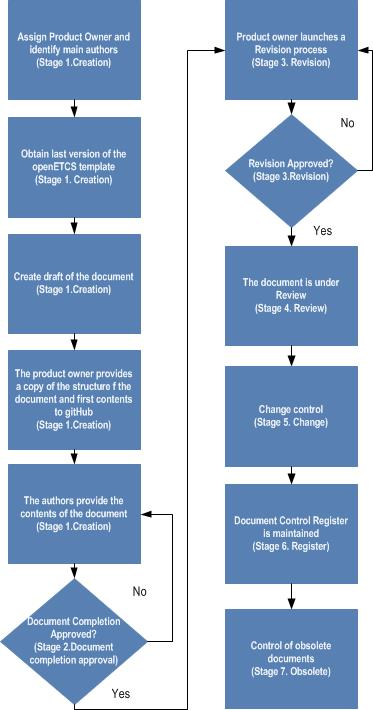
\includegraphics{./figures/DocumentationControlProcess.JPG}
\caption{Documentation Control process flow}
\end{figure}


\subsubsection{Stage One: Creation of the document}

Once the need for a new document is identified the following steps shall be followed to create a new document in a controlled and established way:
\begin{itemize}

\item A Product owner for the new document is identified and assigned as well as the authors and possible main contributors to the document. 
\item The Product owner has the responsibility of checking whether there is a new version of the openETCS template available. The template is stored in the \href{https://github.com/openETCS/ecosystem/tree/master/openETCS_LateX_templates}{[template directory]} of gitHub ant it shall be taken as the starting point for the new document format. In case any requirement is needed and not covered in the current version of the template, a new issue shall be published in the \href{https://github.com/openETCS/ecosystem/issues}{[ecosystem issue tracker]} to request the required additions or changes.
\item The Product owner shall prepare a first draft of the document with a minimum structure of contents and subjects that should be covered in the document. If it applies, some contents shall be provided in several sections.
\item The Product Owner provides the corresponding nomenclature to this first draft following the guidance on nomenclature available in the \href{https://github.com/openETCS/governance/wiki/Nomenclature-Guideline}{[Nomenclature Guideline]}.
\item According to the \href{https://github.com/openETCS/governance/tree/master/SCMP}{[SCMP]} process, the document shall be under control and monitored. The Product Owner shall follow the procedure the process described in that document and shall make the document available in the corresponding directory of a repository in github. In case it is needed, a new directory should be created inside the structure of the repository. 
\item From this moment on, the Product Owner shall work in closely collaboration with the SC Manager to assure that the objectives of the SCMP are met.
\item The Author(s) are informed about the update so they can download the document and begin working with it.
\item The Author(s) provide the contents in the sections assigned in the time estimated by the Product Owner.
\item The document shall be written as such, that it is possible to check the completeness, validity and origin:
\begin{itemize}
\item The document will clearly identify document number, document history, date, description and authorization.
\item All the sections shall be clearly established and identified in the index, as well as the tables and figures used.
\item All referred documents and/or documents which must be read in conjunction shall be identified, with their valid issue.
\item The origin shall be identified with the name of the authors.
\end{itemize}
\end{itemize}

\subsubsection{Stage Two: Document Completion Approval}

\begin{itemize}
\item The Product Owner supervises the writing and completion of the document.
\item The Product Owner decides whether the document is in a stable status and with an adequate level of quality in its contents and subjects covered after making a quick review of the sections included in the document. In that moment, he/she informs the authors that the document has been approved.
\item The SC Manager shall check the format and the nomenclature of the document. 
\end{itemize}

\subsubsection{Stage Three: Revision}

\begin{itemize}
\item The document is ready for Revision. The Product Owner launches a Revision Process and control the process is being carried out according to the established in the Revision Process.
\item The revision process will be carried out in a dedicated Revision Cycle Branch and for a specified period of time where the Committers can add contents or edit them. 
\item The whole process is described in the \href{https://github.com/openETCS/governance/tree/master/Review\%20Process}{[Revision Process Document]}.
\item The Product Owner will complete the document revision, including the update of the Document History section to reflect the changes and current revision status of the document. 
\item Some revisions may include correcting grammar, spelling, and/or formatting errors. The Product Owner is authorized to perform typographical or minor editing corrections such as name changes, title changes, acronym clarifications, etc. without requiring a formal document revision or explicit approval.
\item The SC Manager will control the access to the document and support the approval made by the Product Owner. In this way, the SC Manager shall ensure the document is always available in the expected directory, controls the existence of branches used for the modifications made and verifies the update of the History and version. The SC Manager shall assess the evolution of the document and whether it is in a consistent format.
\item On the other hand, if the document currently being revised and released directly affects any other parent or dependent documents, it is the responsibility of the SC Manager to verify if any affected documents need to be revised.
\end{itemize}

\subsubsection{Stage Four: Review}
\begin{itemize}
\item The review process will be performed against documents already revised and therefore published in the repository. No specific branch for review will be created in the corresponding github repository, and all comments will be made and answered using the Issue Tracker tool available in github.
\item The Product Owner will be assisted by a group of selected Key Customers of the document under review when necessary.
\item The Product Owner will analyze the comments and proceed with their acceptance or rejection.
\item The Product Owner publishes a new version of the document once the process has been completed and  updates the status of the document to “Active”.
\item The Review process is described in detail in the \href{https://github.com/openETCS/governance/tree/master/Review\%20Process}{[Review Process Document]}. 
\item the SC Manager shall ensure the Process is correctly launched and followed by the Product Owner and be responsible for providing any support the Product Owner requires when addressing the review process.
\end{itemize}

\subsubsection{Stage Five: Change Control}
\begin{itemize}
\item Change/Problem Management will ensure standardized methods, processes, and procedures facilitate efficient and prompt handling of all changes, and maintain the proper balance between the need for change and the potential detrimental impact of changes/problems, thus contributing to maintain service level objectives.
\item Whenever a Problem and Change requests is notified to Change/Problem Owner, the Change/Process Management Process is launched. 
\item The Change/Process Management Process is described in detail in the \href{https://github.com/openETCS/governance/tree/master/Change-Problem\%20Process}{[Change/Process Management Process Document]}. 
\item The SC Manager shall ensure the Process is correctly launched and followed by the roles involved and the Product Owner is informed.
\end{itemize}

\subsubsection{Stage Six: Document Control Register}
\begin{itemize}
\item A list of documents shall be maintained in each repository of github so the current status of the document is displayed as well as a quick link to the document, the version, or the Product Owner. More specifically, the following information shall be recorded for each document:
\begin{itemize}
\item Id: a unique identification for the document
\item Title: the complete name provided for the document
\item Version: the last version of the document
\item Owner: the product owner of the document
\item Contributor/Committers/Reviewers: main people involved in the edition and revision/reviewing of the document
\item State: current state of the document (in progress, under revision, under review, released)
\item Delivery: expected date of delivery
\item Folder link: path to the directory in github that contains the document
\end{itemize}
\item The list shall be available in the wiki of each repository of the openETCS project. This wiki page shall be the starting point for any reader that are not aware of the structure of the repository and as a summary of the status of the documents available in that repository.
\item The SC Manager shall be in charge of ensuring the information displayed in the list is accurate and correct as well as maintained whenever it is necessary.
\end{itemize}

\subsubsection{Stage Seven: Control of Obsolete Documents}
\begin{itemize}
\item Those documents that are no longer required, replaced or superseded as determined by the needs of the openETCS project shall be labelled as "Obsolete". 
\begin{itemize}
\item Obsolete documents may be identified as part of the review process and the SC Manager shall be informed about the situation.
\item The Product Owner shall remove the document from the active repository where it has being held until that moment and archive it to prevent unintended use. The Product Owner shall inform the SC Manager about the identification, labelling and moving of the obsolete document found.  
\item An Archived directory shall be available in each repository to contain all the documents qualified as "Obsolete". Those documents must be retained and accessible for the whole evaluation of the openETCS project.
\end{itemize}
\end{itemize}

\end{document}
